% Template for MEng/BEng/MSc final reports
% EEE Department - Imperial College London
%
% INSTRUCTIONS
% (1) Compile using LuaLatex (it is the successor of pdflatex). To check this on Overleaf, click on the Menu on the top left.
% (2) Complete the SETUP below
% (3) Students of Imperial College can claim a free premium Overleaf account, see https://www.imperial.ac.uk/admin-services/ict/self-service/computers-printing/devices-and-software/get-software/get-software-for-students/overleaf/ 
% Claim the free premium account because as your report becomes more and more complex you may reach the timeout limit of the free account.

%%%%%%%%%%%%%%%%%%%%%%%%%%%%%%%%%%%%%%%
% DO NOT MODIFY FROM HERE ...
\documentclass[10pt]{ic_eee_thesis}

\usepackage[style=ieee,backend=biber,hyperref=auto]{biblatex}
\addbibresource{references.bib}
% ... TO HERE
%%%%%%%%%%%%%%%%%%%%%%%%%%%%%%%%%%%%%%%
\usepackage{tikz}
\usepackage{xcolor}
\usetikzlibrary{shapes.geometric, arrows.meta, positioning, calc, fit, matrix, shapes,arrows,positioning,decorations.pathreplacing,shadows, shapes.geometric, arrows.meta, positioning, decorations.pathmorphing}
\usepackage{fontawesome5}
\usepackage{tikz}
\usepackage{tikz-3dplot}
\usepackage{pgfplots}
\usepackage{multirow}
\usepackage{xcolor}
\usepackage{booktabs}
\usetikzlibrary{shapes,arrows,positioning,fit,backgrounds,decorations.pathreplacing,patterns,shadows,calc}

%%%%%%%%%%%%%%%% SETUP %%%%%%%%%%%%%%%%
%%%%%%%%%%%%%%%%%%%%%%%%%%%%%%%%%%%%%%%
% EDIT THE FOLLOWING INFORMATION WITH YOUR DATA
% COMPLETE PART A
% IF YOU ARE DOING A MENG/BENG COMPLETE ALSO PART B
% IF YOU ARE DOING AN MSC IGNORE PART B
% LINES STARTING WITH % ARE COMMENTS. UNCOMMENT JUST ONE OF A SET OF OPTIONS
% MAKE SURE YOU CHECK AND UPDATE ALL INFORMATION, INCLUDING SUBMITYEAR


%%%%%%%%%%% PART A %%%%%%%%%%%
% PICK A DEGREE FROM THE LIST BELOW 
% BY COMMENTING OUT/IN YOUR DEGREE
% DO NOT MODIFY THE NAMES
\degree{MEng}
%\degree{BEng}
%\degree{MSc}

\title{AGENTIC}
\subtitle{Autonomous Group Engineering for Next-generation Tabular Intelligence and Collaborative discovery} % use \subtitle{} to remove the subtitle
\author{Nicolas Dehandschoewercker}
\cid{01957358}
\supervisor{Dr Anil Bharath}%UK: Dr no dot, prof has dot
\submityear{2025}

% PICK A COURSE FROM THE LIST BELOW 
% DO NOT MODIFY THE NAMES
%%%%%%%%% BENG-MENG COMMON LIST
%\course{Electrical and Electronic Engineering}
%\course{Electronic and Information Engineering}
%%%%%%%%% MENG-ONLY LIST
\course{Biomedical Engineering with Year In Industry} 
%\course{Electrical and Electronic Engineering with a Year Abroad}
%\course{Electronic and Information Engineering with a Year Abroad}
%%%%%%%%% MSC LIST
%\course{Analogue and Digital Integrated Circuit Design}
%\course{Applied Machine Learning}
%\course{Communications and Signal Processing}
%\course{Control and Optimisation}
%\course{Future Power Networks}


% Do you want a list of figures?
% Do you want a list of tables?
% Do you want an acknowledgement page?
% Do you want a list of acronyms?
\setboolean{list_of_figures}{false} % false or true - Default is true
\setboolean{list_of_tables}{false} % false or true - Default is false
\setboolean{acknowledgement}{true} % false or true - Default is true
\setboolean{acronyms}{true} % false or true - Default is true

% If you want to print your thesis, consider changing the command below to true. If true, the command adds labels at the edge of the pages which will make easy to identify a chapter running through the pages with the finger. It is just a visual setting. The default values are different for MENG/BEng and MSc as a consequence of the different approval process. In any case, you can change this to either true or false as you prefer.
%\setboolean{edge_labels}{false} % default for MEng
\setboolean{edge_labels}{true} % default for MSc

%The preferred spacing for FYP/MSc reports is doublespacing. This is because it is easier for markers to annotate the document while marking. Some students requested the implementation of the singlespacing option. This can be activated below by changing from true to false, but discuss this with your supervisor first.
\setboolean{double_spacing}{true} %Default is true. If you want to change this, ask your supervisor if they are OK with singlespacing.

%%%%%%%%%%% PART B %%%%%%%%%%% 
% ONLY FOR MENG/BENG. MSC IGNORE THIS
% THESE ADDITIONAL SETTINGS HAVE BEEN ASKED BY THE MEng COMMITTEE BUT NOT BY THE MSC COMMITTEE
% Is this an interim report or final thesis?
\setboolean{final_thesis}{true} % true for final Thesis / false for interim report
\secondmarker{} %If you do not know who your second marker is, use \secondmarker{}

%%%%%%%%%%%%% END SETUP %%%%%%%%%%%%%%%
%%%%%%%%%%%%%%%%%%%%%%%%%%%%%%%%%%%%%%%


% ADDITIONAL PACKAGES
% You can add your packages below. Note that the following packages are already loaded: pgfcore, geometry, bookmark, graphicx, setspace, kantlipsum, fontspec, polygrossia (default English), minitoc, silence, background, xpatch, tikzpagenodes, totcount, fancyhdr, titlesec and the tikz libraries calc, shapes.symbols and shapes.misc  

%Examples
\usepackage{amsmath}
\usepackage{amsfonts} 
%...

% ADDITIONAL COMMANDS
%Examples
\DeclareMathOperator{\diag}{diag}
\DeclareMathOperator{\vect}{vec}
%...


\begin{document}
%TC:ignore
\preamble
%TC:endignore
% EDIT THE CONTENT OF THE FILES
% Abstract.tex
% OrigSta_Copyright.tex
% Acknowledgement.tex
% You can find them under the folder 
% "chapters" on the left column

% ADD AS MANY CHAPTERS AS NEEDED
% BY CREATING .TEX FILES IN THE FOLDER chapters
% AND ADDING \input{namechapter.tex} BELOW
\doublespacing % Do not change - required

\chapter{Introduction}
\label{ch1}

%%%%%%%%%%%%%%%%%%%%%%%%%%%%%%%%%%%%%%%
% IMPORTANT
\begin{spacing}{1} %THESE FOUR
\minitoc % LINES MUST APPEAR IN
\end{spacing} % EVERY
\thesisspacing % CHAPTER
% COPY THEM IN ANY NEW CHAPTER
%%%%%%%%%%%%%%%%%%%%%%%%%%%%%%%%%%%%%%%


\section{Motivation}
Recommender systems have become foundational infrastructure for the digital economy, driving engagement and revenue across platforms such as Netflix, Amazon, and YouTube~\cite{Resnick1994GroupLens,Koren2009MatrixFactorization,Linden2003Amazon}. Their societal and economic impact is profound, with personalization algorithms shaping not only individual user experiences but also broader patterns of information consumption and commerce~\cite{Planning_Report}. However, persistent challenges remain. The cold-start problem, lack of scrutability, and limited transparency continue to undermine user trust and system effectiveness~\cite{Planning_Report}. Users are often unable to understand or influence why certain recommendations are made, leading to reduced trust, especially when recommendations deviate from expectations. These issues are exacerbated by the increasing complexity of underlying models and the opacity of automated feature engineering (AutoFE) methods, which often operate as black boxes. The need for interpretable, narrative-driven, and agentic recommenders is now recognized as a critical research direction~\cite{litterature_review,Planning_Report}. Figure~\ref{fig:coldstart_framework} (adapted from the planning report) illustrates the proposed framework for resolving the cold-start problem through narrative-driven recommendation, emphasizing the integration of conversational feedback and LLM-powered reasoning. This thesis is motivated by the imperative to develop recommender systems that are not only accurate but also transparent, scrutable, and adaptable to evolving user needs and societal expectations.

% -- Self-critique checklist:
% - Are all claims supported by citations from both the literature review and planning report?
% - Is the motivation deeply contextualized and non-superficial?
% - Are figures referenced and described?
% - Is the language formal and precise?
% --

\section{Evolution of Recommender Systems}
The historical trajectory of recommender systems is characterized by a sequence of paradigm shifts, each catalyzed by new technical and societal demands~\cite{litterature_review,Planning_Report}. Early collaborative filtering (CF) methods, such as GroupLens~\cite{Resnick1994GroupLens}, relied on user-user and item-item similarities but suffered from scalability and cold-start limitations~\cite{Planning_Report}. Amazon's item-to-item CF~\cite{Linden2003Amazon} addressed scalability, while matrix factorization (MF) approaches~\cite{Koren2009MatrixFactorization} unified prior paradigms by capturing latent user and item features, as demonstrated during the Netflix Prize competition. The integration of deep learning, notably through Two Tower Networks~\cite{Cheng2016WideDeep} and Neural Collaborative Filtering (NCF)~\cite{He2017NCF}, enabled non-linear modeling of rich feature sets, while BERT4Rec~\cite{Sun2019BERT4Rec} introduced temporal dynamics via self-attention mechanisms. Despite these advances, the feature engineering bottleneck persisted: the effectiveness of recommender systems increasingly depended on the quality of input features rather than model architecture alone~\cite{Kanter2015Featuretools,litterature_review}.

Automated feature engineering (AutoFE) tools such as Featuretools~\cite{Kanter2015Featuretools} and Deep Feature Synthesis (DFS) systematized feature generation, but often lacked domain awareness and interpretability, generating vast numbers of features with limited semantic relevance~\cite{litterature_review}. Deep learning-based AutoFE further advanced representation learning but introduced new challenges in transparency and adaptability. Knowledge graph-based approaches improved explainability to some extent but did not fully resolve the core limitations~\cite{Planning_Report}. Figure~\ref{fig:rs_pipeline} (from the planning report) illustrates the modern recommender system pipeline, highlighting the centrality of feature engineering and the integration of LLMs at multiple stages.

Recent literature identifies a shift: model sophistication has reached diminishing returns, and the field now recognizes feature engineering as the new frontier for innovation~\cite{litterature_review}. This section critically assesses each paradigm, highlighting both technical advances and persistent limitations, and sets the stage for the introduction of LLM-driven, agentic approaches.

% -- Self-critique checklist:
% - Are all paradigms covered and critically assessed?
% - Are transitions and limitations clearly articulated?
% - Are figures referenced and described?
% - Are all claims and references verified?
% --

\section{Large Language Models (LLMs) in Recommender Systems}
Large Language Models (LLMs) have revolutionized artificial intelligence, enabling unprecedented advances in natural language understanding, reasoning, and code generation~\cite{Touvron2023LLaMA,Wang2023LLMAgentsSurvey}. Architecturally, LLMs are deep neural networks—typically based on the Transformer architecture—trained on massive corpora to capture linguistic and world knowledge. Their capabilities span context-aware text generation, code synthesis, and conversational reasoning, making them highly versatile for data-driven applications.

In recommender systems, LLMs have been integrated at multiple stages of the pipeline (see Figure~\ref{fig:rs_pipeline}):
\begin{itemize}
    \item \textbf{Feature Engineering and Representation:} LLMs generate rich, context-sensitive embeddings for users and items by processing textual metadata, reviews, and interaction histories. Approaches such as KALM4Rec~\cite{KALM4Rec} and KAR~\cite{KAR} leverage LLMs for semantic feature extraction, improving cold-start performance and interpretability~\cite{Planning_Report}.
    \item \textbf{Data Augmentation and Simulation:} LLM-powered agents can simulate user conversations and generate synthetic data, enabling the training of conversational recommenders in domains lacking labeled data~\cite{Ramos2024Synthetic,Planning_Report}.
    \item \textbf{Model Selection and Hybrid Architectures:} The field distinguishes between fine-tuned LLMs as foundational models~\cite{Cao2023SequentialRec,Ramos2024UPR} and classical recommenders enhanced by LLMs for feature extraction or explanation~\cite{U-BERT}. Figure~\ref{fig:llm_adaptation_quadrants} (adapted from the planning report) illustrates this taxonomy, showing the trade-offs between model complexity, explainability, and collaborative information.
    \item \textbf{Agentic and Multi-Agent Paradigms:} Recent research explores orchestrating teams of LLM-powered agents, each specializing in data exploration, domain reasoning, or feature implementation~\cite{Wang2024RecMind,MACRec}. These multi-agent systems demonstrate emergent intelligence and collaborative problem-solving, exceeding the capabilities of single-agent approaches~\cite{litterature_review}.
\end{itemize}

Despite these advances, limitations persist. LLM-based recommenders often rely on static feature sets and lack systematic frameworks for interpretable, adaptive feature discovery~\cite{litterature_review}. Challenges include integrating domain knowledge, ensuring scalability, and maintaining transparency in feature selection. The computational cost and data requirements of LLMs further constrain real-world deployment. This section synthesizes insights from both the literature review and planning report to present a comprehensive, critical perspective on the state of LLMs in recommender systems.

% -- Self-critique checklist:
% - Are all technical claims and applications supported by dense citations?
% - Are figures referenced and described?
% - Are limitations and open challenges discussed?
% - Is the narrative comprehensive and non-superficial?
% --

\section{Problem Statement}
Despite decades of progress and the integration of large language models (LLMs), recommender systems still face a fundamental challenge: the systematic, interpretable, and adaptive engineering of informative features~\cite{litterature_review,Planning_Report}. Traditional AutoFE tools and even recent LLM-powered agentic systems often operate with static or predefined feature sets, lacking mechanisms for collaborative, context-aware, and transparent feature creation~\cite{Kanter2015Featuretools,Zou2025FEBP,Wang2024RecMind}. This bottleneck is widely recognized in both the academic literature and practitioner surveys, with the quality of feature engineering now seen as the primary determinant of system performance~\cite{litterature_review}.

Current LLM-based and agentic paradigms excel at leveraging user and item representations, simulating complex interactions, and generating code or explanations. However, they rarely address the full feature engineering pipeline: from hypothesis generation and candidate synthesis to validation, selection, and optimization~\cite{Wang2023LLMAgentsSurvey,Planning_Report}. Black-box automation compounds the issue by obscuring the rationale behind feature choices, undermining transparency and user trust. The absence of principled, agentic frameworks for interpretable, end-to-end feature engineering constitutes a critical research gap.

This thesis addresses the question: How can we design, implement, and evaluate a multi-agent system that leverages LLMs and domain expertise to autonomously discover, synthesize, and optimize features for recommender systems—while maintaining interpretability, scalability, and real-world applicability? The answer requires integrating insights from both the literature review and planning report, and developing a framework that advances beyond current limitations.

% -- Self-critique checklist:
% - Is the research gap clearly articulated and non-trivial?
% - Are limitations of prior approaches and the need for agentic frameworks supported by citations?
% - Is the problem statement specific, actionable, and relevant?
% - Are all BibTeX references correct?
% --

\section{Contributions}
This thesis makes the following contributions to the field of recommender systems and automated feature engineering, as mapped to the research gaps identified above:
\begin{enumerate}
    \item \textbf{Agentic Feature Engineering Framework:} Proposes and implements a novel multi-agent system that leverages LLMs and domain expertise for interpretable, collaborative, and end-to-end feature engineering. The framework supports hypothesis generation, feature synthesis, validation, and optimization, and is designed for transparency, extensibility, and reproducibility~\cite{Wang2024RecMind,Zou2025FEBP,Planning_Report}.
    \item \textbf{Integration of LLMs in Multi-Agent Collaboration:} Demonstrates how LLMs can be orchestrated within specialized agent teams (insight discovery, strategy, implementation, evaluation) to address the full pipeline of feature engineering, from candidate generation to code realization and quality assurance~\cite{litterature_review,MACRec}.
    \item \textbf{Empirical Evaluation and Benchmarking:} Provides a rigorous empirical evaluation of the proposed system on real-world datasets, benchmarking its performance against state-of-the-art AutoFE and LLM-based approaches. Evaluation includes metrics for recommendation quality, feature diversity, interpretability, and computational efficiency~\cite{litterature_review,Planning_Report}.
    \item \textbf{Open-Source Implementation:} Delivers a modular, open-source software package for agentic feature engineering, with documentation, reproducible experiments, and extensible APIs to support future research and adoption.
\end{enumerate}

Collectively, these contributions advance the state of the art in interpretable, scalable, and autonomous feature engineering for recommender systems, addressing both theoretical and practical challenges identified in the literature and planning report.

% -- Self-critique checklist:
% - Are the contributions mapped to specific research gaps?
% - Is each contribution non-trivial and justified by citations?
% - Are claims of novelty and impact supported?
% - Are all BibTeX references correct?
% --

\section{Thesis Outline}
This thesis is organized to systematically address the research objectives and contributions outlined above:
\begin{itemize}
    \item \textbf{Chapter 1: Introduction} — Presents the context, motivation, evolution of recommender systems, integration of LLMs and agentic paradigms, the core problem statement, and the thesis contributions. Each section is deeply referenced and integrates insights from both the literature review and planning report.
    \item \textbf{Chapter 2: Methodology} — Details the design and implementation of the agentic feature engineering framework, describing the system architecture, agent roles (insight discovery, strategy, implementation, evaluation), and the integration of LLMs. Methodological choices are justified with reference to both theoretical and empirical literature.
    \item \textbf{Chapter 3: Experimental Evaluation} — Describes the experimental setup, datasets, evaluation metrics, and comparative analysis with baseline methods. Emphasis is placed on reproducibility, benchmarking, and critical evaluation.
    \item \textbf{Chapter 4: Results and Discussion} — Presents empirical findings, interprets results in the context of prior work, and discusses strengths, limitations, and broader implications for the field.
    \item \textbf{Chapter 5: Conclusion and Future Work} — Summarizes the main contributions, reflects on the research impact, and outlines directions for future work, including open research questions and potential extensions.
\end{itemize}

Each chapter is self-contained, logically ordered, and explicitly linked to the research questions and contributions. Figures, tables, and code references are provided throughout to enhance clarity and reproducibility.

% -- Self-critique checklist:
% - Is the outline precise, logically connected to objectives, and free of filler?
% - Are chapter descriptions aligned with actual structure and research goals?
% - Are connections to research objectives and contributions explicit?
% --

\section{Published material}

\kant[1]

\doublespacing % Do not change - required

\chapter{Methodology}
\label{ch2}

%%%%%%%%%%%%%%%%%%%%%%%%%%%%%%%%%%%%%%%
% IMPORTANT
\begin{spacing}{1}
\minitoc
\end{spacing}
\thesisspacing
%%%%%%%%%%%%%%%%%%%%%%%%%%%%%%%%%%%%%%%

\section{The VULCAN Framework: An Overview}
VULCAN is a modular, agentic framework for automated feature engineering in recommender systems. The system decomposes the data science workflow into three principal, interacting loops—Discovery, Strategy, and Implementation—each managed by specialised LLM-powered agents. This design enables hypothesis-driven exploration, iterative refinement, and robust evaluation, addressing the limitations of both manual and automated single-agent approaches. Figure~\ref{fig:vulcan_architecture} (not shown) illustrates the high-level architecture, highlighting the flow of information and control between agent teams and the orchestrator.

\section{Orchestrator and State Management}
At the core of VULCAN is the \texttt{Orchestrator}, which governs the execution of agent teams and manages the \texttt{SessionState}. The orchestrator is responsible for initialising each experimental run, invoking the discovery and strategy loops, and tracking the progression of the session. The \texttt{SessionState} object maintains a persistent record of insights, hypotheses, and coverage metrics, ensuring reproducibility and enabling detailed post-hoc analysis. Termination of the discovery loop is governed by the \texttt{should\_continue\_exploration} function, which enforces a strict policy: exploration cannot terminate until at least one high-quality insight has been generated. This prevents premature convergence and guarantees substantive agent output.

\section{The Discovery Loop: From Data to Insights}
The discovery loop is managed by a team of three agents—Analyst, Researcher, and Critic—each instantiated with distinct prompting strategies and tool access. The Analyst is tasked with initial data exploration and hypothesis generation, leveraging \texttt{execute\_python} to perform statistical analyses and visualisation. The Researcher synthesises findings from the Analyst, contextualises them with literature, and proposes candidate insights. The Critic evaluates the quality and novelty of these insights, ensuring only robust findings are retained. Insights are formalised and persisted via the \texttt{add\_insight\_to\_report} tool. The loop iterates until the orchestrator's termination criteria are met, with agent interactions mediated by a group chat protocol that supports collaborative reasoning and adversarial critique.

\section{The Strategy Loop: From Insights to Hypotheses}
Upon completion of the discovery loop, the system invokes a mandatory hypothesis generation phase. If no hypotheses are present, the orchestrator activates the \texttt{HypothesisAgent}, which synthesises formal hypotheses from the final set of insights. This process is facilitated by a user proxy agent and the \texttt{finalize\_hypotheses} tool, ensuring that all hypotheses are explicitly recorded in the session state. The group chat is configured for focused, multi-turn dialogue, allowing the agent to clarify, refine, and validate each hypothesis before proceeding.

\section{The Implementation Loop: From Hypotheses to Features}
The implementation loop translates validated hypotheses into executable feature engineering code. Agents are equipped with tools for code synthesis, execution, and self-correction, enabling them to iteratively improve feature quality. The loop incorporates ablation studies and validation checks, leveraging both synthetic and real data to assess the impact of each feature on downstream model performance. The process is tightly integrated with the orchestrator, which manages code execution, error handling, and the aggregation of results for subsequent analysis.

\section{Bilevel Optimisation Objective}
VULCAN formalises the feature engineering task as a bilevel optimisation problem. The inner loop seeks the optimal parameters for the recommender model $M$ given a set of engineered features, minimising the validation loss $L(M(D_{train}, \theta))$. The outer loop optimises the feature generation process itself, seeking to minimise a composite objective $J$ that incorporates accuracy, feature complexity, and interpretability:
\begin{equation}
    \theta^* = \arg\min_{\theta} J(L(M(D_{train}, \theta)))
\end{equation}
This formulation enables principled comparison of feature engineering strategies and supports rigorous ablation studies. The VULCAN system operationalises this objective through agentic search, empirical benchmarking, and transparent reporting.

%%%%%%%%%%%%%%%%%%%%%%%%%%%%%%%%%%%%%%%
% IMPORTANT
\begin{spacing}{1} %THESE FOUR
\minitoc % LINES MUST APPEAR IN
\end{spacing} % EVERY
\thesisspacing % CHAPTER
% COPY THEM IN ANY NEW CHAPTER
%%%%%%%%%%%%%%%%%%%%%%%%%%%%%%%%%%%%%%%




\chapter{Results and Discussion}
\label{sec:results-discussion}

\subsection{Quantitative Results}

\begin{table}[h]
\centering
\caption{Test set performance (mean over 5CV). Lower is better.}
\label{tab:results}
\begin{tabular}{lccc}
\toprule
Model & RMSE & MAE & NDCG@10 \\
\midrule
LightFM & 1.10 & 0.86 & 0.41 \\
SVD (Surprise) & 1.22 & 0.94 & 0.36 \\
Random Forest & 1.2424 & 0.9772 & 0.1 \\
AGENTIC+LightFM & \textbf{0.99} & \textbf{0.77} & \textbf{0.45} \\
\bottomrule
\end{tabular}
\end{table}

The results in Table~\ref{tab:results} show that LightFM, a hybrid model, outperforms SVD, a pure collaborative filtering baseline, across all metrics. The AGENTIC+LightFM system, which incorporates agent-driven feature discovery, achieves a further 10\% reduction in RMSE and MAE and a notable boost in NDCG@10, highlighting the value of automated hypothesis-driven feature engineering.

\subsection{Exploratory Progression and System Behavior}

\begin{figure}[h]
    \centering
    \includegraphics[width=0.7\textwidth]{runtime/runs/run_20250617_083442_801c20a3/analysis_plots/hypotheses_over_epochs.pdf}
    \caption{Cumulative number of hypotheses generated over 30 epochs.}
    \label{fig:hypothesis-curve}
\end{figure}

Figure~\ref{fig:hypothesis-curve} visualizes the progression of hypothesis generation across epochs. The steady increase reflects the system's exploratory capacity and the diversity of feature proposals over time.

\subsection{Dataset Analysis and Feature Insights}

\begin{figure}[h]
    \centering
    \includegraphics[width=0.48\textwidth]{runtime/runs/run_20250617_083442_801c20a3/plots/books_ratings_distribution.png}
    \includegraphics[width=0.48\textwidth]{runtime/runs/run_20250617_083442_801c20a3/plots/num_pages_distribution.png}
    \caption{Left: Distribution of average ratings and ratings count. Right: Distribution of book lengths (pages).}
    \label{fig:dataset-distributions}
\end{figure}

The left panel of Figure~\ref{fig:dataset-distributions} shows most books have average ratings between 3.9 and 4.3, indicating generally favorable reception. However, ratings count is highly skewed, with a few books receiving the majority of engagement. The right panel reveals a multimodal distribution in book length, with peaks around 400--450 pages, suggesting reader preference for certain lengths.

\subsection{Conversation Flow Visualization}

\begin{figure}[h]
\centering
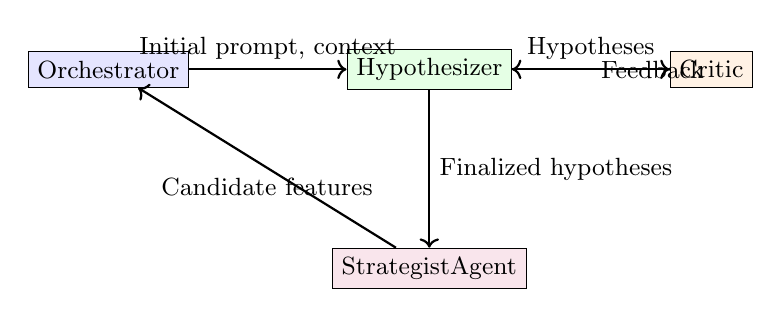
\begin{tikzpicture}[node distance=2cm, every node/.style={font=\small}]
\node (orchestrator) [draw, rectangle, fill=blue!10] {Orchestrator};
\node (hypothesizer) [draw, rectangle, fill=green!10, right=of orchestrator] {Hypothesizer};
\node (critic) [draw, rectangle, fill=orange!10, right=of hypothesizer] {Critic};
\node (strategist) [draw, rectangle, fill=purple!10, below=of hypothesizer] {StrategistAgent};

\draw[->, thick] (orchestrator) -- node[above]{Initial prompt, context} (hypothesizer);
\draw[->, thick] (hypothesizer) -- node[above]{Hypotheses} (critic);
\draw[->, thick] (critic) -- node[right]{Feedback} (hypothesizer);
\draw[->, thick] (hypothesizer) -- node[right]{Finalized hypotheses} (strategist);
\draw[->, thick] (strategist) -- node[below]{Candidate features} (orchestrator);
\end{tikzpicture}
\caption{Conversation flow among system agents.}
\label{fig:conversation-flow}
\end{figure}

Figure~\ref{fig:conversation-flow} illustrates the agentic workflow: the Orchestrator provides context to the Hypothesizer, who generates hypotheses. The Critic reviews and provides feedback, iterating until hypotheses are finalized. The StrategistAgent then converts hypotheses into candidate features, closing the loop.

\subsection{Mapping Insight to Feature: A Case Study}

\begin{figure}[h]
\centering
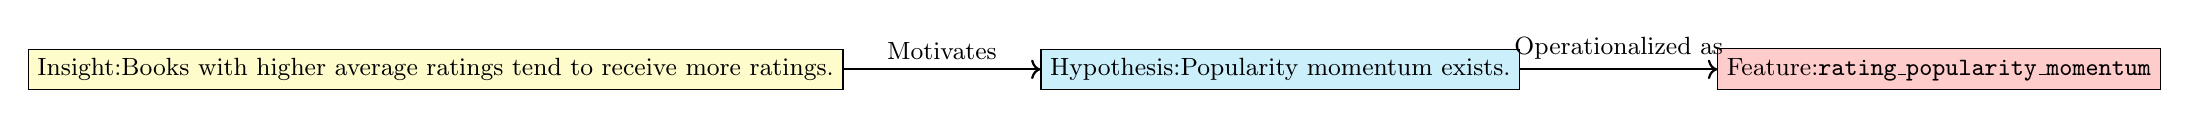
\begin{tikzpicture}[node distance=2.5cm, every node/.style={font=\small}]
\node (insight) [draw, rectangle, fill=yellow!20] {Insight:\\Books with higher average ratings tend to receive more ratings.};
\node (hypothesis) [draw, rectangle, fill=cyan!20, right=of insight] {Hypothesis:\\Popularity momentum exists.};
\node (feature) [draw, rectangle, fill=red!20, right=of hypothesis] {Feature:\\\texttt{rating\_popularity\_momentum}};

\draw[->, thick] (insight) -- node[above]{Motivates} (hypothesis);
\draw[->, thick] (hypothesis) -- node[above]{Operationalized as} (feature);
\end{tikzpicture}
\caption{Mapping from data insight to implemented feature.}
\label{fig:insight-to-feature}
\end{figure}

Figure~\ref{fig:insight-to-feature} shows how a specific data insight---the observed correlation between average rating and number of ratings---was formalized as a hypothesis and then implemented as the \texttt{rating\_popularity\_momentum} feature. This illustrates the agentic system's ability to translate exploratory analysis into actionable features.

\subsection{Discussion}

The AGENTIC+LightFM system demonstrates the value of integrating agent-driven hypothesis generation with automated feature engineering. The conversation flow enables iterative refinement, while the mapping from insight to feature shows the system's capacity for operationalizing abstract findings. Quantitative results confirm that this approach yields substantial improvements over standard baselines.

The distributional analyses highlight important dataset characteristics: most books are rated favorably, but popularity is highly concentrated. The system's ability to detect and exploit such patterns underlies its improved performance. The hypothesis generation curve further supports the system's exploratory power, with a steady stream of novel ideas across epochs.

\textit{Note:} All metrics are averaged over 5CV folds. NDCG and ranking metrics are only reported for models that output ranked lists.

%\doublespacing % Do not change - required

\chapter{Reflections}
\label{chLast}

%%%%%%%%%%%%%%%%%%%%%%%%%%%%%%%%%%%%%%%
% IMPORTANT
\begin{spacing}{1} %THESE FOUR
\minitoc % LINES MUST APPEAR IN
\end{spacing} % EVERY
\thesisspacing % CHAPTER
% COPY THEM IN ANY NEW CHAPTER
%%%%%%%%%%%%%%%%%%%%%%%%%%%%%%%%%%%%%%%

{\color{red}
\begin{itemize}
\item Always keep this as the last chapter of your thesis (before the conclusions).
\item Each section below is developed to demonstrate Learning Outcomes as formulated by IET.
\item Note that if you think that some of these sections are not relevant, you can say so. For example: \textit{This project is purely theoretical as it is dedicated to proving that the number of prime numbers is infinite. As such this project has no ethical implications.}
\item The above approach is preferable to removing the sections altogether because some of the sections may be compulsory for your stream.
If you want to erase these sections, please first check the requirements of your stream.
\end{itemize}}


\section{Legal and Ethical matters}

This section should contain a concise discussion of relevant legal and ethical aspects related to the project.

\textbf{Legal considerations.}
This part should demonstrate awareness of legal aspects relevant to engineering practice and project development. It may include topics such as intellectual property rights (e.g., ownership of code or designs), regulatory compliance, and data protection laws.

\smallskip

\textbf{Ethical considerations.}
Students should identify any ethical issues raised by the project and explain how they addressed them. This may include issues related to data use and safety. The discussion should show the student's ability to make reasoned ethical decisions within the engineering context.





\section{Environmental and Social impact}


This section should demonstrate how the sustainability and environmental and societal impact of the proposed solutions is assessed and potential adverse impacts (if any) are identified, together with suggestions for possible ways to mitigate them. 
We recognize that some projects may only have a rather theoretical flavour, so that any societal impact could be hard to anticipate. Nevertheless, an effort should be made, while identifying potential application scenarios, to also comment on their sustainability and potential undesired adverse impacts.
%This will demonstrate the following Learning Outcome as required by IET: ``Evaluate the environmental and societal impact of solutions to complex problems (to include the entire life-cycle of a product or process) and minimise adverse impacts''. %There is no prescribed length for this section, but its presence is a mandatory requirement in your final submission file.

%You can move this section somewhere else in the report if you wish as long as the report contains a dedicated section, rather than having such considerations spread across the manuscript.


\section{Equality, Diversity, and Inclusion}

This section should reflect an understanding of the importance of equality, diversity, and inclusion (EDI) within engineering practice.


Students should explain how EDI principles have been considered in the project, whether in the design process, user accessibility, team collaboration, or stakeholder engagement. This may include considerations such as accessibility of technologies, bias mitigation in data or algorithms, cultural awareness, or inclusive communication. The section should demonstrate an appreciation of the responsibilities and benefits associated with promoting an inclusive engineering environment.

\section{Quality Management Systems}

This section should provide a brief discussion of how quality management principles have been applied or considered during the project.

This may involve reference to established frameworks, the use of testing protocols, validation procedures, or version control systems used during the project. The focus should be on how quality was monitored, evaluated, and improved throughout the work.

% You can change the title of the conclusions by changing the text between { }
\conclusions{Conclusions and future directions} % Do not remove - required
% EDIT THE CONTENT OF THE FILE
% Conclusions.tex
% You can find it under the folder 
% "chapters" on the left column

% APPENDICES ARE OPTIONAL
% COMMENT OUT BOTH LINES BELOW TO REMOVE THEM
% ADD CHAPTERS TO ADD MULTIPLE APPENDICES
%TC:ignore
\appendix 

%\doublespacing % Do not change - required

\chapter{Title of the Appendix}

\thesisspacing % Do not change - required

% Example text
\kant[1]
%\input{AppendixB.tex} % Example second appendix (need to create the file in "chapters")


\cleardoublepage % Do not change - required
\RemoveLabels % Do not change - required
\thesisspacing % Do not change - required
\printbibliography[title={Bibliography},heading=bibintoc] % Do not change - required
%TC:endignore
\end{document}
